\subsubsection{Multiple Features}
\begin{itemize}[--]
	\item Instead of just one feature ($x$), we known multiple features ($x_1,\ldots, x_n$). eg. size, number of bedrooms, number of floors, age of home.
	\item $x^{(i)}_j:$ value of feature $j$ in $i^{th}$ training example
	\item Now our hypothesis must account for multiple features: 
		$$h_\theta (x)=\theta_0 + \theta_1 x_1 + \ldots \theta_n x_n$$
	\item Again we define $x_0 = 1$ to simplify future math ($x^{(i)}_0=1$).
	$$x=\begin{bmatrix} x_1\\ \vdots\\ x_n\end{bmatrix}\in \mathbb{R}^{n+1}\text{,  }
		\theta = \begin{bmatrix}\theta_0 \\ \vdots\\ \theta_n\end{bmatrix}\in\mathbb{R}^{n+1}$$
	\item Transposing the $\theta$ vector given our assumption for $x_0^{(i)}$ allows us to simplify our hypothesis into:
		$$h_\theta (x) = \theta^{T}x$$
\end{itemize}

\subsubsection{Gradient Descent for Multiple Variables}
\begin{itemize}[--]
	\item Repeat until convergence ($j=0,\ldots, n$): 
		$$\theta_j := \theta_j \alpha\frac{1}{m}\sum_{i=1}^{m}(h(x^{(i)}-y^{(i)}))x^{(i)}_j$$
	\item This is a valid generalization of the previous formula because of our base case $x^{(i)}_0=1$
\end{itemize}

\subsubsection{Gradient Descent in Practice I - Featuer Scaling}
\begin{itemize}[--]
	\item \textbf{Feature scaling:} if features are on similar scales then we converge more quickly
	\item Your parameters will oscillate along the larger ranged parameter making it's way much slower towards the center (in the case of two variables); whereas, if both axis were equal then you don't have a worst case to fret about
	\begin{center}
		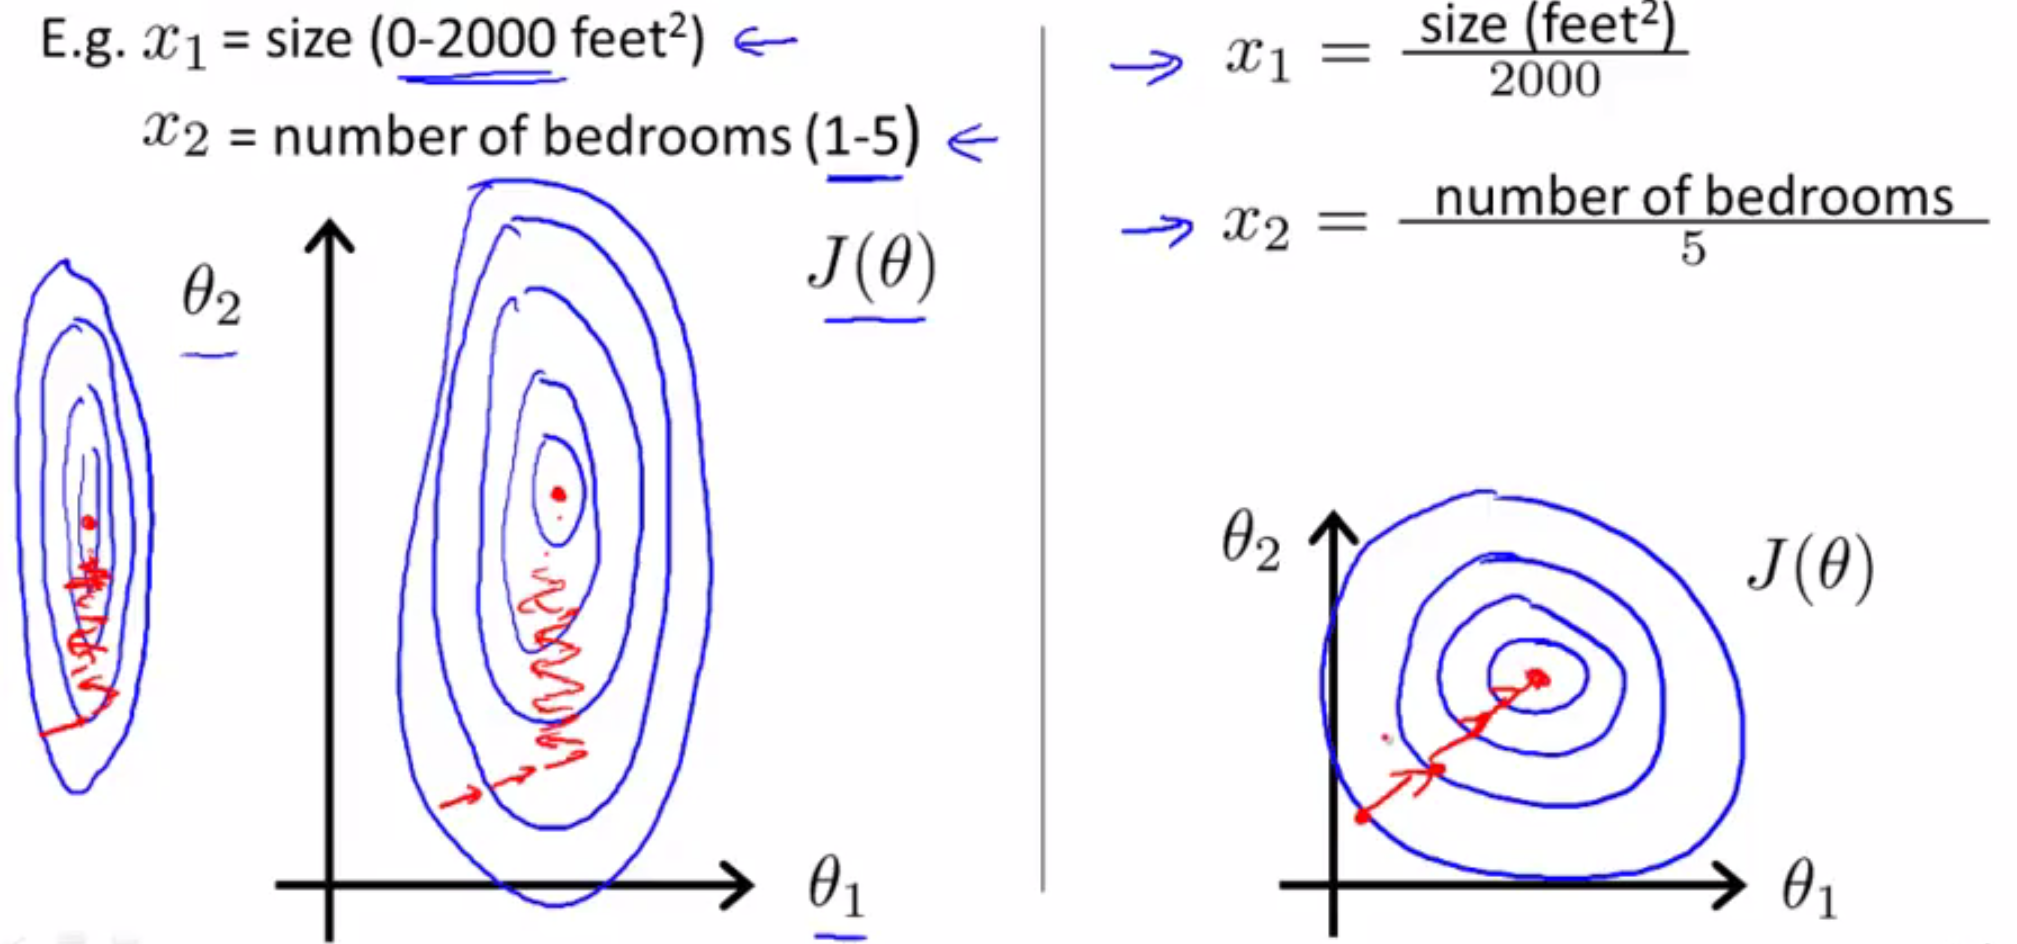
\includegraphics[scale=0.25]{sections/cs229/w2/feature_scaling.png}
	\end{center}

	\item Typically, we want to scale each feature into approximately a $-1\leq x_i \leq 1$ range (same order of magnitude).
	\item \textbf{Mean normalization:} replacing $x_i$ with $x_i-\mu_i$ to make features have approximately zero mean (does not apply to $x_0=1$).
	\item Combining mean normalization and feature scaling we assign $x_i := \frac{x_i-\mu_i}{range_i}$

\end{itemize}

\subsubsection{Gradient Descent in Practice II - Learning Rate}
\begin{itemize}[--]
	\item To ensure gradient descent is working correctly, plot the cost function against the number of iterations. It should converge towards 0, decreasing at every iteration.
	\item The number of iterations required can vary widely for different applications
	\item You can create an automatic convergence test to ensure appropriately ending of gradient descent by checking if the difference between two iterations $\epsilon$ is below a threshold.
	\item If there is any increase in slope, use a smaller $\alpha$
	\item For sufficiently small $\alpha$, $J(\theta )$ should decrease on every iteration
	\item But if $\alpha$ is too small, gradient descent an be slow to converge
	\item To choose $\alpha$ try: $\ldots, 0.001, 0.003, 0.01, 0.03, 0.1, 0.3, 1,\ldots$
\end{itemize}

\subsubsection{Features and Polynomial Regression}
\begin{itemize}[--]
	\item Suppose we have a housing price prediction: $h(x)=\theta_0 + \theta_1 (frontage)+\theta_2 (depth)$
	\item We can define a new feature $(area)=(frontage)(depth)$, that we can use in a new hypothesis $h(x)=\theta_0+\theta_1 (area)$
	\item We can map these hypothesis of more complex features into a linear regression problem: 
	\begin{align*}
		h(x)&=\theta_0 + \theta_1 x_1 + \theta_2 x_2 + \theta_3 x_3    
  		  	&=\theta_0 + \theta_1 (size) + \theta_2 (size)^2 + \theta_3 (size)^3
	\end{align*}

	\item If your features are like those chosen, then feature scaling is very important
	\item There are many more choices for modifications to our features (such as: $\sqrt{}$).
	\item Trying new features can allow you to have a more appropriate model
\end{itemize}

\subsubsection{Normal Equations}
\begin{itemize}[--]
	\item The \textbf{normal equation} allows us to solve for $\theta$ analytically (without iterations)
	\item Intuition: $J(\theta) = a\theta^2+b\theta+c$
	In previous calculus classes you would find the minimum by taking the derivative set equal to 0 and solving for $\theta$. 
	\item This can be extended with partial fractions and solving for every $\theta_j\in\theta$. $$\frac{\partial}{\partial\theta_j}J(\theta)=\ldots=0 \text{    (for every}j\text{)}$$
	\item We construct a matrix from the features and a vector from the solutions as so ($n$ features, $m$ examples):

	\[X=\begin{bmatrix}
		x_0^{(1)} & x_1^{(1)} & \dots & x_n^{(1)} \\
		x_0^{(2)} & x_1^{(2)} & \dots & x_n^{(2)} \\
		\vdots & \vdots & \ddots & \vdots \\
		x_0^{(m)} & x_1^{(m)} & \dots x_n^{(m)} 
	\end{bmatrix} \in \mathbb{R}^{m\times (n+1)}
	 \]

	 \[
	y=\begin{bmatrix}
		y^{(1)} \\
		y^{(2)} \\
		\vdots \\
		y^{(m)}
	\end{bmatrix}\in \mathbb{R}^{m\times 1}
	 \]

	 \item We can then represent the $\theta$ by the \textbf{normal equation} $$\theta = (X^{T}X)^{-1}X^{T}y$$\
	 \item $X$ is entitled the \textbf{design matrix}
	 \item Normal equation does not perform well with a large $n$ due to the computation $(X^{T}X)^{-1}\in\mathbb{n\times n}$ which is typically $\O{n^3}$
\end{itemize}